
\hypertarget{hello}{%
\section{Hello!}\label{hello}}

This is the Rmarkdown document!\\
But surprise: It is linked to overleaf via Github!

And this is a line:

\begin{Shaded}
\begin{Highlighting}[]
\KeywordTok{plot}\NormalTok{(}\DecValTok{1}\OperatorTok{:}\DecValTok{100}\NormalTok{, }\DecValTok{1}\OperatorTok{:}\DecValTok{100}\NormalTok{)}
\end{Highlighting}
\end{Shaded}

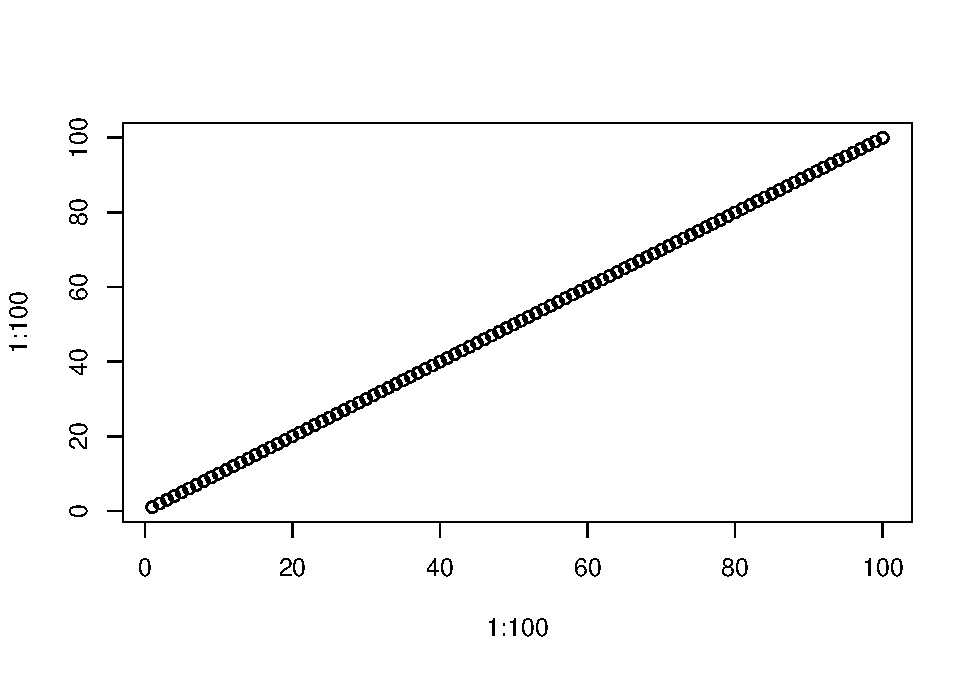
\includegraphics{rmd_files/figure-latex/unnamed-chunk-1-1.pdf}

You can knit this document, which will create a .tex file. Before you
push it to Github, you have to run

\texttt{./trimtex.sh\ filename.tex}

in the shell!

Then you can push the document!

